% AstroRegolith manuscript — formatted for npj Microgravity (Article).
%
% Every number in the Results is read from a table in ../results/tables/ and every
% figure from ../results/figures/, both regenerated by `bash scripts/run_all.sh`.
% references.bib is generated by scripts/check_references.py from Crossref.
% See BUILD.md for how to build, and for swapping in the publisher's class file.

\documentclass[11pt,a4paper]{article}

\usepackage[utf8]{inputenc}
% lmodern must precede fontenc: it supplies scalable Type 1 outlines in place of
% the default bitmap Computer Modern. Without it microtype's font expansion
% aborts with "auto expansion is only possible with scalable fonts" on a minimal
% TeX installation, which is exactly what the CI image is.
\usepackage{lmodern}
\usepackage[T1]{fontenc}
\usepackage[margin=2.4cm]{geometry}
\usepackage{graphicx}
\usepackage{booktabs}
\usepackage{amsmath}
\usepackage{siunitx}
\usepackage[hidelinks]{hyperref}
\usepackage[numbers,sort&compress]{natbib}
\usepackage{authblk}
\usepackage{caption}
\usepackage{microtype}
\usepackage{lineno}

\captionsetup{font=small,labelfont=bf}
\graphicspath{{figures/}}
\sisetup{detect-weight=true,per-mode=symbol}
\linenumbers

\title{\bfseries Growth-anchored transcriptomics of \textit{Arabidopsis thaliana}
in Apollo lunar regolith, and an open database for regolith plant science}

\author[1]{Richard J. Barker}
\affil[1]{Center of Space Exploration (CoSE)}
\date{}

\begin{document}
\maketitle

\begin{abstract}
\noindent
Growing food beyond Earth means growing it in regolith, and the evidence base for
doing so is small, scattered and hard to pool. We assembled every regolith-relevant
dataset in NASA's two open repositories --- nine biological studies in the Open
Science Data Repository (OSDR) and six physical-science investigations in the
Physical Sciences Informatics (PSI) system --- and found that only two carry plant
imagery and that PSI holds no plant-in-regolith data at all. Within that record, one
study is uniquely informative: OSD-476, in which \textit{Arabidopsis thaliana} was
grown in \SI{900}{\milli\gram} of Apollo 11, 12 and 17 regolith against a JSC-1A
simulant control. Its deposited metadata keys each RNA-seq sample to a growth plate
and to a twelve-timepoint leaf-count trajectory, which makes it possible --- and, to
our knowledge, unprecedented for this dataset --- to relate expression to how each
individual plant actually grew rather than only to which regolith it grew in. Joining
the sequenced plants to their own growth (twelve one-to-one joins, four plate-mean
joins; Spearman $\rho=0.84$ between two independently measured phenotype layers), we
find 2\,008 genes correlated with leaf-emergence rate at 5\% FDR, of which 299 replicate
within the Apollo samples alone, where substrate no longer tracks growth. Eighty-two of
those genes are invisible to the published substrate contrasts. They are enriched for
hormone catabolism and cell communication, and include the developmental timer
\textit{SPL3}, the DELLA \textit{RGL1}, the auxin oxidase \textit{DAO1} and the
ER-body myrosinase-associated \textit{PBP1}. We release the catalogue, the harmonised
phenotype and expression tables, the analysis code and a static community database
that lets any laboratory contribute calibrated regolith imagery through a free phone
application. The clearest practical finding is a metadata one: OSD-476's growth-anchored
reanalysis was possible only because someone recorded a plate and a leaf count against
each sequenced plant, and four of its twenty samples are excluded from that analysis
because nobody photographed them.
\end{abstract}

\noindent\textbf{Keywords:} lunar regolith; regolith simulant; \textit{Arabidopsis thaliana};
in-situ resource utilisation; transcriptomics; phenotyping; open data; ISA-Tab

\section{Introduction}

The case for regolith agriculture is an arithmetic one. Every kilogram of soil launched
to the Moon competes with a kilogram of something else, so a habitat that grows food
will grow it in what is already there. The question is not whether regolith can support
plant growth --- it can --- but at what cost to the plant, and whether that cost can be
engineered away.

Paul, Elardo and Ferl provided the first and still the only direct answer using returned
lunar material, germinating \textit{Arabidopsis thaliana} in Apollo 11, 12 and 17
regolith \citep{paul2022apollo}. Plants grew, but slowly, with severe stress
morphologies and transcriptomes indicative of ionic, salt, metal and reactive-oxygen
stress. The lunar samples are irreplaceable; the experiment will not be repeated at
scale. Everything else the field knows comes from simulants, whose relationship to real
regolith is itself a research question --- LHS-1, a lunar highlands simulant, carries
\SI{15.8}{\percent} more Al\textsubscript{2}O\textsubscript{3} and
\SI{19.8}{\percent} less FeO by weight than the mare soil returned by Chang'e-5
\citep{exolithlhs1,li2022change5}.

That makes pooling what exists unusually valuable and unusually difficult. Regolith
studies are deposited across repositories designed for different communities, described
in different vocabularies, and reported with substrate provenance that ranges from a
batch number to a trade name. Meanwhile the analytical convention in the field is to
contrast treatment groups: Apollo 11 versus Apollo 12 versus simulant. That convention
discards information the deposits already contain. In OSD-476, growth varied by more
than two orders of magnitude in rosette area \emph{within} the regolith-grown plants,
from \SI{0.14}{\milli\metre\squared} to \SI{16.1}{\milli\metre\squared}, and one Apollo 11
plant never produced a true leaf at all. Treating those plants as replicates of a single
condition throws away the very gradient that distinguishes a plant coping from a plant
failing.

Here we do three things. We catalogue the regolith slice of NASA's open repositories and
say plainly what is and is not in it. We use the per-plant metadata deposited with
OSD-476 to anchor its transcriptomes to measured growth, and ask which genes track how
a plant fared rather than where its substrate came from. And we release the result as a
static, server-free database that others can read, cite and add to.

\section{Results}

\subsection{The regolith record across two NASA repositories is small, and two-thirds
of it has no imagery}

Searching OSDR for regolith, simulant and Apollo terms and inspecting every returned
study's file listing yields nine biological datasets
(Supplementary Table~S1; \texttt{public/data/osdr\_regolith\_catalog.json}). They span
returned Apollo material (OSD-476, OSD-855, OSD-877, OSD-883), lunar and Martian
simulants (OSD-856, OSD-581), asteroid simulant (OSD-670), a microbial Mars-analogue
study (OSD-305) and one terrestrial ionic-stress proxy (OSD-22, high magnesium). Only
two --- OSD-476 and OSD-670 --- deposit plant photographs, 83 images in total. The
remainder deposit metadata, tabular results or sequence data alone, which limits how far
their phenotypes can be re-measured or pooled.

The Physical Sciences Informatics system returns six investigations relevant to a
regolith grower, but none of them involve plants in regolith. They cover granular
mechanics in microgravity (STRATA-1, PSI-110), regolith-derived cement as an ISRU
feedstock (PSI-83, PSI-84, PSI-174), cabin dust behaviour (PSI-47) and capillary water
delivery to roots (PSI-187). This is worth stating explicitly, because the physics that
governs how a regolith bed packs, drains and sheds dust is exactly what a growth study
has to design around, and it currently lives in a repository most plant biologists do
not search.

\subsection{Substrate behaviour separates regolith from soil more sharply than
composition alone suggests}

Probe measurements on eight candidate substrates while water was added
(Fig.~\ref{fig:substrate}a--c) show a lunar simulant reaching \SI{35.5}{\percent}
water content at an electrical conductivity of \SI{25}{\micro\siemens\per\centi\metre},
against \SI{13.5}{\percent} and \SI{64}{\micro\siemens\per\centi\metre} for potting
soil. The nutrient contrast is starker still: over the whole run the lunar simulant
released no detectable nitrogen, phosphorus or potassium on the probe's scale, where
potting soil registered 43, 0 and 30 respectively. Mechanically disturbing the same
simulant (`stirred') raised its apparent nitrogen from 0 to 20 and its potassium from
0 to 13, which is a useful reminder that regolith's nutrient availability is a function
of handling as much as of chemistry.

Composition then adds a second axis. Comparing the LHS-1 highlands simulant against
Chang'e-5 mare soil (Fig.~\ref{fig:substrate}d) shows systematic, terrain-driven gaps:
LHS-1 is richer in Al\textsubscript{2}O\textsubscript{3} (+\SI{15.8}{wt\percent}),
SiO\textsubscript{2} (+\SI{9.0}{wt\percent}) and Na\textsubscript{2}O
(+\SI{2.6}{wt\percent}), and poorer in FeO (\SI{-19.8}{wt\percent}), MgO
(\SI{-4.9}{wt\percent}) and TiO\textsubscript{2} (\SI{-4.4}{wt\percent}). Iron and
titanium are precisely the elements implicated in the ionic and oxidative stress
regolith-grown plants display, so a simulant choice is not a neutral logistical
decision --- it sets the magnitude of the stress under test.

\begin{figure}[t]
\centering
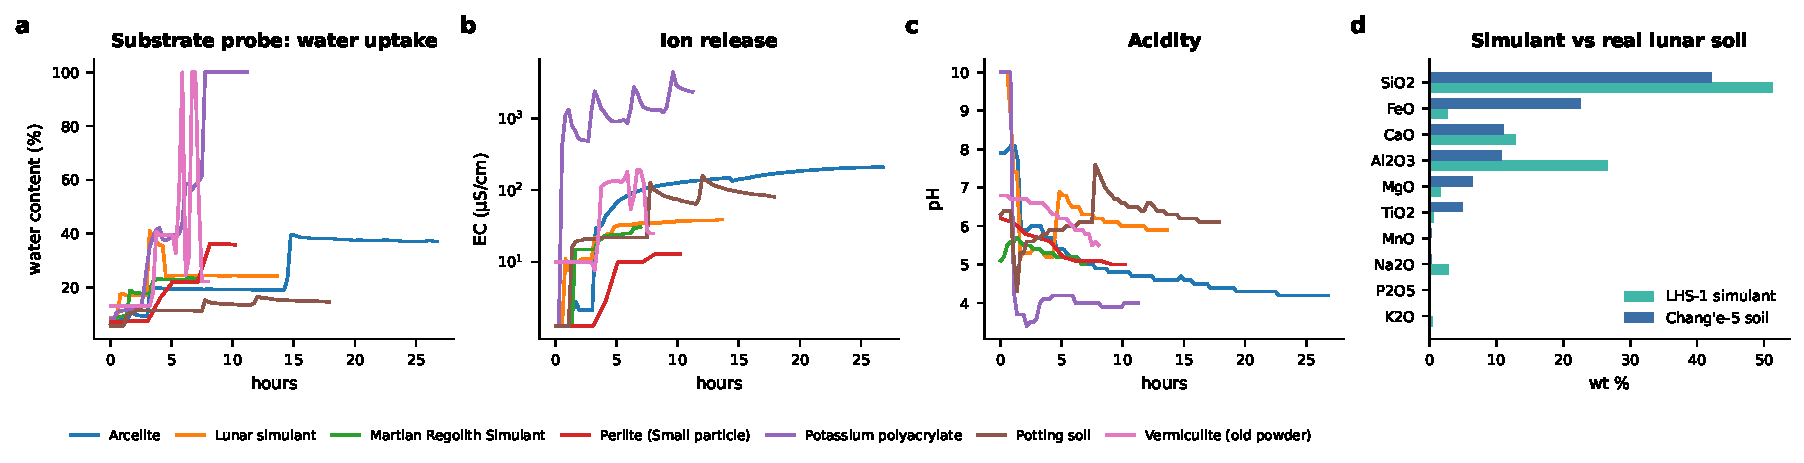
\includegraphics[width=\textwidth]{fig2_substrate_characterisation.pdf}
\caption{\textbf{What a regolith substrate does and what it is made of.}
(a--c) Soil-probe response of eight substrates as water was added to
\SI{15}{\milli\litre} of each: water content, electrical conductivity and pH.
(d) Bulk oxide chemistry of the LHS-1 lunar highlands simulant against Chang'e-5
returned mare soil \citep{exolithlhs1,li2022change5}. Data:
\texttt{results/tables/substrate\_*.csv}.}
\label{fig:substrate}
\end{figure}

\subsection{Every sequenced plant in OSD-476 can be joined to its own growth}

OSD-476's ISA-Tab archive contains a morphometric assay file that records, for sixteen
of the twenty RNA-seq samples, the growth plate the plant occupied (P1--P4), the plate
scans it appears in, and a twelve-timepoint leaf count. Because each plate carried
exactly one Apollo 11, one Apollo 12 and one Apollo 17 plant, those twelve lunar
samples join one-to-one to an individual plant. The four phenotyped JSC-1A samples
share a plate with three further control plants and are joined to the plate mean. The
remaining four JSC-1A replicates carry no morphometrics at all and are excluded rather
than imputed.

A second, independent phenotype layer comes from PlantCV shape traits re-scored from
the same plate scans \citep{gehan2017plantcv}: 133 plant-days across 28 plants and five
imaging days, converted from pixels to millimetres using the scale factors carried in
the trait table. The two layers were measured differently and agree strongly
(Spearman $\rho = 0.843$, $p = 4.2\times10^{-5}$, $n = 16$; Fig.~\ref{fig:growth}c),
which is a check on the join rather than a consequence of it.

Growth separates the substrates cleanly (Fig.~\ref{fig:growth}a,b; Table~\ref{tab:growth}).
JSC-1A plants put out a first true leaf on day 4 after the first plate scan and reached
$9.0 \pm 0.8$ leaves and $45.9 \pm 17.1$~\si{\milli\metre\squared}; Apollo 11 plants
waited until day 10.7 and reached $2.0 \pm 1.6$ leaves and
$0.84 \pm 1.13$~\si{\milli\metre\squared}. Apollo 12 and 17 sit between, and overlap
each other. Rosette area dips between the day-2 and day-4 scans in every regolith
group, coinciding with the thinning to one seedling per well that the study protocol
records for days 6--8; the Apollo plants recover from it far more slowly than the
controls.

\begin{figure}[t]
\centering
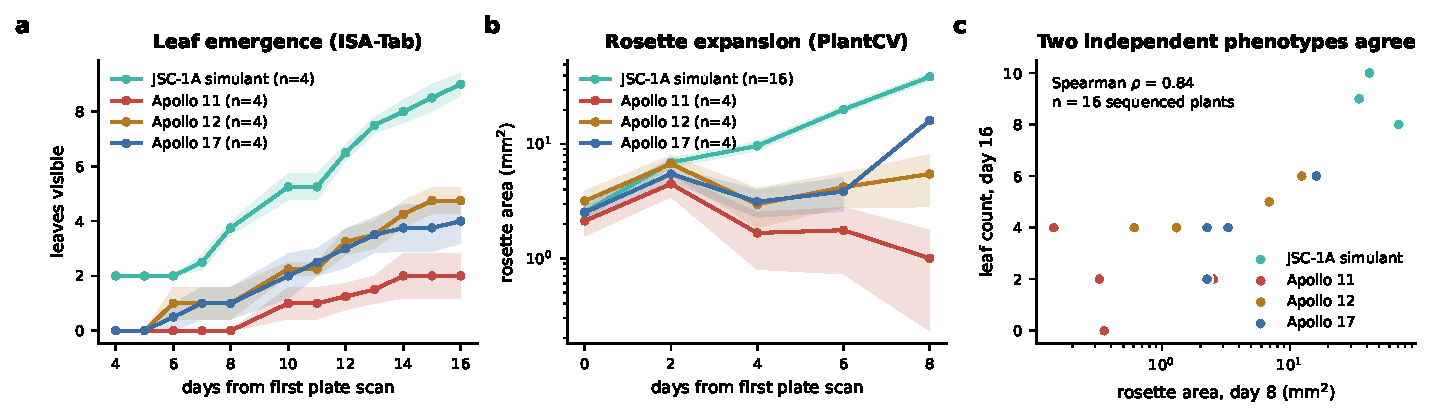
\includegraphics[width=\textwidth]{fig1_growth_phenotypes.pdf}
\caption{\textbf{Two independent phenotype layers for the sequenced plants.}
(a) Leaf counts from the OSD-476 ISA-Tab morphometric assay, mean $\pm$ s.e.m.
(b) Rosette area re-scored from the same plate scans with PlantCV (log scale).
(c) The two layers against each other for the sixteen phenotyped RNA-seq samples.
Time is expressed as days from the first plate scan; see Methods for why no sowing
date is published.}
\label{fig:growth}
\end{figure}

\begin{table}[t]
\centering
\small
\caption{Growth of the sixteen phenotyped OSD-476 plants, by substrate. Mean $\pm$ s.d.;
$n=4$ per substrate. Leaf counts are from the deposited ISA-Tab assay; rosette area is
the PlantCV re-score on the last morphometric day. Source:
\texttt{results/tables/sample\_phenotype\_expression\_map.csv}.}
\label{tab:growth}
\begin{tabular}{lccccc}
\toprule
Substrate & $n$ & Day of first leaf & Final leaves & Leaf rate (d$^{-1}$) & Rosette area (\si{\milli\metre\squared}) \\
\midrule
JSC-1A simulant   & 4 & 4.0  & $9.00 \pm 0.82$ & 0.66 & $45.88 \pm 17.07$ \\
Apollo 11 regolith & 4 & 10.7 & $2.00 \pm 1.63$ & 0.21 & $0.84 \pm 1.13$ \\
Apollo 12 regolith & 4 & 8.0  & $4.75 \pm 0.96$ & 0.43 & $5.30 \pm 5.50$ \\
Apollo 17 regolith & 4 & 8.5  & $4.00 \pm 1.63$ & 0.37 & $5.98 \pm 6.78$ \\
\bottomrule
\end{tabular}
\end{table}

\subsection{Anchoring expression to growth recovers genes the substrate contrasts miss}

We correlated variance-stabilised expression of 23\,533 genes against six growth
covariates, in two analyses (Methods). The \emph{primary} analysis uses all sixteen
phenotyped plants and is the more powerful, but growth and substrate are confounded in
it: every JSC-1A plant outgrew every Apollo plant. The \emph{within-lunar} analysis uses
the twelve Apollo plants alone, where growth still spans 0--6 leaves and
0.14--16.1~\si{\milli\metre\squared} but the simulant contrast is gone. A gene
significant in both, with a consistent sign, is tracking growth rather than substrate.

Leaf-emergence rate is the most productive covariate: 2\,008 genes at 5\% FDR in the
primary analysis and 395 within the Apollo samples, against 114 and 0 for rosette area
(Fig.~\ref{fig:growth_tx}a; Supplementary Table~S2). Across all covariates, 361
gene--covariate pairs covering 299 distinct genes are significant in both analyses with
a consistent sign (Fig.~\ref{fig:growth_tx}b). Of those 299 genes, 217 also appear among
the 8\,458 differentially expressed in at least one published Apollo-versus-JSC-1A
contrast --- and 82 do not (Fig.~\ref{fig:context}a). Those 82 are the return on
anchoring to growth: genes whose expression tracks the gradient of plant performance
without differing enough between treatment groups to survive a group contrast.

The strongest growth-tracking genes are developmental and hormonal rather than
stress-response genes (Fig.~\ref{fig:growth_tx}d--f). \textit{SPL3}
(AT2G33810, $\rho = +0.95$ with final leaf number), a squamosa-promoter-binding-like
factor that times the juvenile-to-adult transition downstream of miR156
\citep{wu2009spl}, is the single most strongly correlated gene. \textit{RGL1}
(AT1G66350, $\rho = +0.95$ with leaf rate) encodes a DELLA protein
\citep{sananmishra2016della}. \textit{DAO1} (AT1G14130, $\rho = -0.93$), the
dioxygenase that oxidises indole-3-acetic acid \citep{porco2016dao1}, and the auxin-transport
kinase \textit{PID} (AT2G34650, $\rho = +0.93$) sit on either side of auxin homeostasis,
and the cytokinin oxidase \textit{CKX7} (AT5G21482), one of the family whose
over-expression phenocopies cytokinin deficiency \citep{werner2003ckx}, appears among the
positively correlated set.
The defence side is equally coherent: \textit{PBP1}/\textit{JAL30} (AT3G16420) and
\textit{BGLU23}/\textit{PYK10} (AT3G09260), both ER-body proteins of the myrosinase
system \citep{nakano2017pyk10}, correlate negatively with growth, as does the circadian
and cold-responsive \textit{COR27} (AT5G42900).

GO-slim over-representation (Fig.~\ref{fig:context}b) matches that reading. Genes
positively correlated with leaf rate are enriched for catalytic activity
($1.2\times$, $q = 0.018$), oxoacid metabolism ($2.0\times$, $q = 0.018$) and response
to abiotic stimulus ($2.7\times$, $q = 0.031$). Genes negatively correlated --- the ones
higher in the plants that fared worst --- are enriched for cell communication
($3.8\times$, $q = 0.020$ in the robust set; $3.3\times$, $q = 0.031$ within the Apollo
samples), with signal transduction, glutathione metabolism and secondary metabolism
following just below the corrected threshold. This is a growth--defence trade-off drawn
along a continuous axis rather than inferred from a two-group comparison.

\begin{figure}[t]
\centering
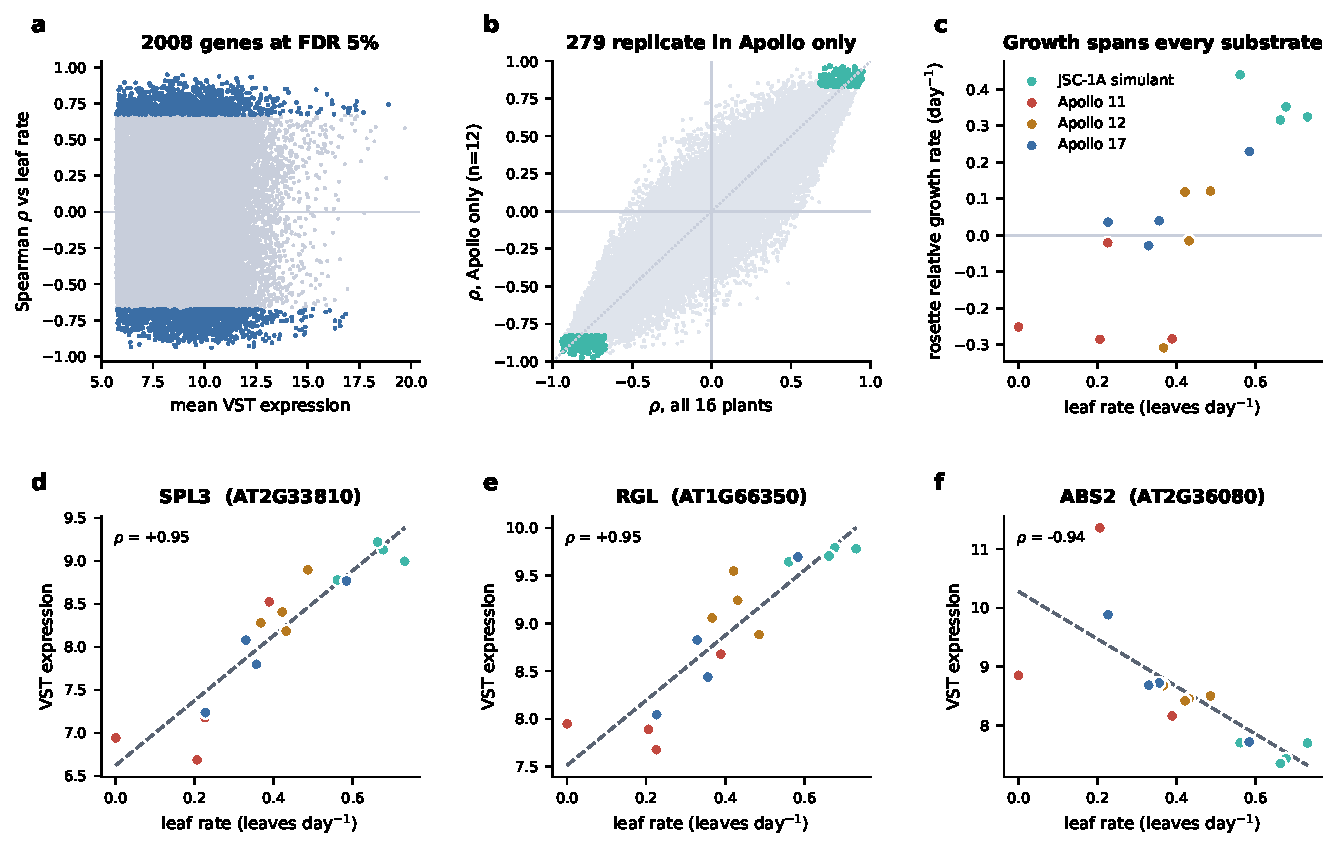
\includegraphics[width=\textwidth]{fig3_growth_anchored_transcriptomics.pdf}
\caption{\textbf{Growth-anchored transcriptomics.}
(a) Spearman $\rho$ against leaf rate versus mean expression; blue, 5\% FDR. Plotting
against expression rather than $p$ is deliberate: with fixed $n$, $p$ is a deterministic
function of $|\rho|$, so a volcano would show only its own geometry.
(b) $\rho$ in the primary analysis against $\rho$ in the Apollo-only analysis, all genes;
teal, significant in both with a consistent sign.
(c) The two growth covariates against each other, coloured by substrate.
(d--f) Example genes. Data: \texttt{results/tables/growth\_correlated\_genes.csv}.}
\label{fig:growth_tx}
\end{figure}

\begin{figure}[t]
\centering
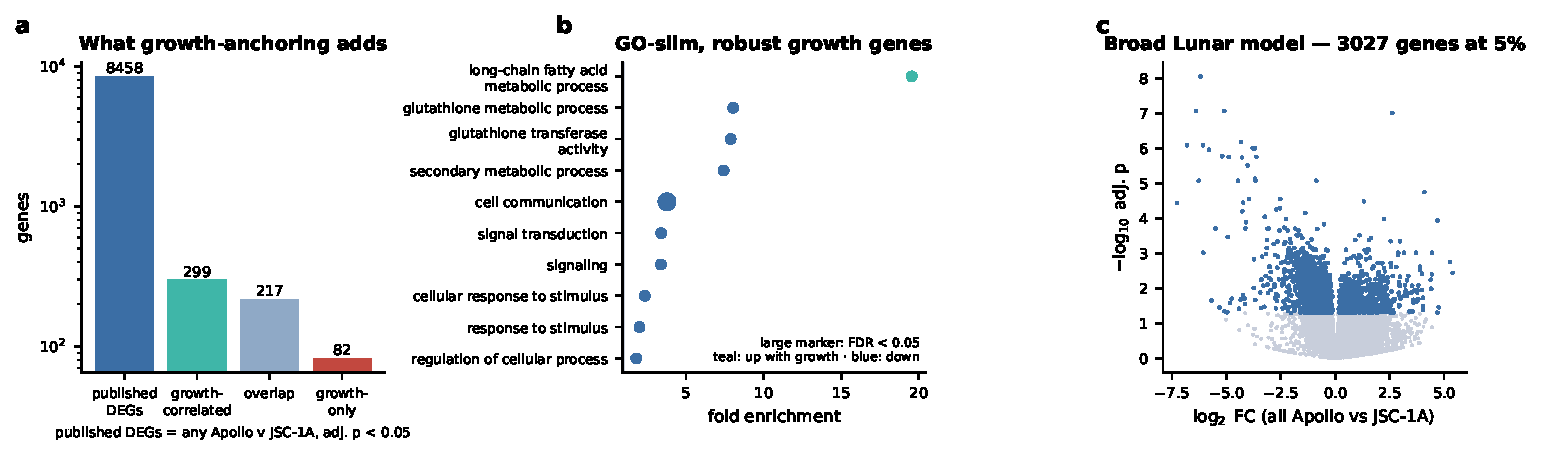
\includegraphics[width=\textwidth]{fig4_context_and_enrichment.pdf}
\caption{\textbf{What growth-anchoring adds, and to what.}
(a) Published differentially expressed genes (any Apollo versus JSC-1A contrast,
adjusted $p<0.05$) against the robust growth-correlated set, their overlap, and the
genes found only by anchoring to growth.
(b) GO-slim over-representation for the robust set; large markers pass 5\% FDR.
(c) The Broad Lunar model --- all Apollo samples pooled against JSC-1A in one linear
model --- 3\,027 of 21\,594 genes at adjusted $p<0.05$ (887 up, 2\,140 down in regolith).}
\label{fig:context}
\end{figure}

\subsection{An open, server-free database for the regolith community}

The catalogue, the harmonised tables and the analysis are published as a static site
(\url{https://dr-richard-barker.github.io/AstroRegolith/}) that runs entirely in the
reader's browser. Neither NASA API permits cross-origin requests --- OSDR answers
\texttt{Access-Control-Allow-Origin: osdr.nasa.gov} and PSI runs the same backend ---
so the site reads JSON harvested offline by the accompanying scripts, which keeps every
displayed figure traceable to a committed table and lets the whole resource be hosted
for nothing.

Contribution uses Epicollect5 \citep{aanensen2014epicollect}, a free data-collection
application. A contributor photographs a plant beside a calibration marker carrying four
ArUco fiducials and a fifteen-chip colour reference; the marker is detected in the
reader's browser to recover \si{\milli\metre} per pixel and a colour correction, so an
ordinary phone photograph becomes a measurement rather than an illustration. The
supplied form asks for the substrate fields that determine reusability --- simulant
name, supplier \emph{batch}, blend ratio, particle size, pre-treatment --- and for days
after sowing and leaf count, chosen deliberately to match OSD-476's own metadata so that
a contributed series can be plotted on the same axes as the Apollo plants.

\section{Discussion}

The result we would most like the field to take from this work is not a gene list. It is
that OSD-476's growth-anchored reanalysis exists only because somebody recorded a plate
identifier and a leaf count against each sequenced plant, and that four of its twenty
samples are excluded from that reanalysis because nobody photographed them. In a study
using irreplaceable Apollo material, a 20\% loss of analysable samples was avoidable
with a camera. The deposited metadata also contains a discrepancy we could not resolve:
the ages at harvest and leaf counts admit no single sowing date consistent with all
samples, so all growth here is reported on days from the first plate scan. We report
that rather than silently choosing one of the two candidate dates.

The gene-level findings should be read with matching care. The developmental timer
\textit{SPL3} correlating almost perfectly with final leaf number is close to a positive
control --- a plant with more leaves is further along the same developmental programme
\textit{SPL3} reports on --- and it is reassuring precisely because it recovers something
already known. The hormone-catabolism genes are more interesting: \textit{DAO1} and
\textit{CKX7} govern the removal of auxin and cytokinin rather than their synthesis, and
both track growth. That points at hormone \emph{turnover} as a place where regolith
stress is registered, which is testable by direct hormone quantification and was
predicted, from pathway modelling alone, in the earlier analysis this repository
supersedes.

\textit{RGL1} needs an explicit caveat. It encodes a DELLA protein, and DELLA
stabilisation under stress is a long-standing explanation for the dwarfed, delayed
phenotypes that regolith-grown plants share with gibberellin mutants
\citep{achard2006della,sananmishra2016della,colebrook2014ga}. It is tempting to read
$\rho = +0.95$ as support for that model. It is not: DELLA activity is controlled
principally by GA--GID1-dependent protein degradation rather than transcript abundance
\citep{sun2011della}, and gibberellin signalling feeds back on \textit{RGL}
transcription, so a transcript correlation is consistent with several opposite
mechanisms. What we can say is that a DELLA transcript is among the
most tightly growth-coupled genes in this dataset, in both analyses, which makes DELLA
protein quantification in regolith-grown plants a well-motivated next experiment rather
than a settled conclusion. The same caution applies to the wider inversion hypothesis
--- that removing green-revolution dwarfing alleles might suit crops to regolith
\citep{wu2020grf4della,hedden2020ga} --- which this dataset motivates but cannot test.

The limitations are substantial and worth stating plainly. Sixteen plants is a small
sample for genome-wide correlation, and the standard deviations underlying our power
estimates are themselves poorly determined at $n=4$ per substrate. Growth and substrate
are confounded in the primary analysis; the within-lunar analysis breaks that
confounding but at reduced power, which is why rosette area yields no robust hits.
GO-slim over a background of roughly 1\,900 terms is conservative at this sample size,
so the enrichment we report is a floor rather than a survey. And the whole analysis
rests on a single study --- because, as the catalogue above shows, there is currently no
second study with returned lunar material, paired transcriptomes and per-plant
phenotypes to replicate it in. Building that second study, and the third, is what the
contribution workflow is for.

\section{Methods}

\subsection{Data sources}
OSDR studies were catalogued by searching the OSDR API for regolith, simulant, lunar,
Martian and asteroid terms, seeded with a curated accession list because the
relevance-ranked search omits several historic Apollo-era deposits, then re-reading each
study's file listing so that counts are measured rather than asserted. Study descriptions
came from the OSDR biodata API. PSI investigations were retrieved from the PSI GeoDE
search endpoint. OSD-476's ISA-Tab archive, sample table, contrast table, variance-stabilised
counts and differential-expression table --- the last produced by the GeneLab pipeline with DESeq2
\citep{love2014deseq2} --- were downloaded from OSDR \citep{berrios2021genelab,osdr476}. PlantCV shoot traits, the pooled Broad Lunar linear
model, and the substrate-probe runs were taken from the project's precursor repository.
All retrieval is scripted and idempotent (\texttt{scripts/00}--\texttt{02},
\texttt{scripts/10}).

\subsection{Phenotype harmonisation}
Leaf counts were parsed from the ISA-Tab morphometric assay file
(\texttt{a\_OSD-476\_morphometric-analysis\_image-analysis\_imagej.txt}), giving twelve
timepoints between 2021-05-06 and 2021-05-18 for sixteen samples. PlantCV traits were
converted from pixels to millimetres using the \texttt{linear\_scale} and
\texttt{area\_scale} columns carried in the source table, after asserting that
\texttt{area\_scale} equals \texttt{linear\_scale}$^2$; two contours whose treatment
group was unassignable were dropped at QC. Imaging dates were taken from the image
filenames and cross-checked against the source table's day-of-month column.

No sowing date is published. For each sample the candidate harvest dates are the imaging
days whose leaf count equals the deposited leaf count at collection, each implying a
sowing date of harvest minus age at harvest; because all plants shared a chamber, one
date must fit all of them. The intersection is empty --- the Apollo samples (21 d) imply
2021-04-27 and JSC-1A replicate 3 (20 d) implies 2021-04-28 --- so growth is reported on
days from the first plate scan (2021-05-02), and the per-sample candidates are published
in \texttt{results/tables/sowing\_date\_check.csv}.

\subsection{Sample-to-plant join}
Each RNA-seq sample was joined to its plate from the morphometric assay and to plants of
the same substrate on that plate. Apollo samples join one-to-one; JSC-1A samples join to
the mean of the four control plants on their own plate; samples without morphometrics are
labelled \texttt{unlinked} and excluded. The join is asserted in code: exactly twelve
one-to-one joins, four plate-mean joins over four plants each, and four unlinked samples,
or the pipeline fails.

\subsection{Growth-anchored correlation}
Six covariates were derived per plant: final leaf count, OLS slope of leaf count against
day, day of first true leaf, area under the leaf-count curve,
$\log_{10}$ rosette area on the last morphometric day, and relative growth rate of
rosette area. Variance-stabilised counts (rRNA-removed, as deposited) were filtered to
23\,533 genes with non-zero variance across the sixteen phenotyped samples. Spearman
$\rho$ and its $t$-approximation $p$ were computed gene-wise by a vectorised rank
correlation validated against \texttt{scipy.stats.spearmanr}, with genes whose ranks are
fully tied within a subset excluded rather than divided by zero. $p$-values were adjusted
by Benjamini--Hochberg \citep{benjamini1995fdr} within each analysis $\times$ covariate.
The robust set comprises gene--covariate pairs significant at 5\% FDR in both the primary
and within-lunar analyses with the same sign of $\rho$.

\subsection{Functional enrichment}
GO-slim annotations were taken from the \texttt{GOSLIM\_IDS} column OSDR ships with the
GLDS-476 differential-expression table, so no external mapping is introduced. Terms with
at least five annotated genes in the tested background were assessed by a one-sided
hypergeometric test against the background of tested, annotated genes, with
Benjamini--Hochberg control within each gene set. Term names were resolved from the EBI
QuickGO service and cached.

\subsection{Reproducibility}
\texttt{bash scripts/run\_all.sh} regenerates every table, figure and site dataset from
the primary sources; retrieval steps are idempotent and analysis steps are deterministic.
Dependencies are pinned in \texttt{requirements.txt}. \texttt{references.bib} is generated
from Crossref by \texttt{scripts/check\_references.py}, which resolves every DOI and fails
the build on an unresolved one, so no citation in this manuscript is written from memory.

\section*{Data availability}
All derived tables, figures and site datasets are in the accompanying repository
(\url{https://github.com/dr-richard-barker/AstroRegolith}) and archived on Zenodo.
Primary data remain with their depositors: NASA OSDR \citep{osdr476,osdr670}, NASA PSI
\citep{nasapsi}, and the Exolith Lab simulant specification \citep{exolithlhs1}. Files
retrieved but not redistributed --- chiefly the 36~MB GLDS-476 differential-expression
table --- are listed in \texttt{MANIFEST.tsv} with their source URL, retrieval date and
checksum, and are re-fetched by the pipeline.

\section*{Code availability}
Analysis code is MIT-licensed and in \texttt{scripts/}; the database application is in
\texttt{src/}. Derived data, figures and text are CC-BY-4.0 \citep{astroregolith}.

\section*{Acknowledgements}
This work builds directly on the OSD-476 deposit of A.-L. Paul, S. M. Elardo and
R. J. Ferl, whose decision to record per-plant morphometrics alongside the sequencing
made the central analysis possible.

\section*{Competing interests}
The author declares no competing interests.

\bibliographystyle{unsrtnat}
\bibliography{references}

\end{document}
